\chapter{Attack Narrative}
In this chapter, we go through the process of exploiting the Wreath network, providing reproduceable steps of the entire exploitation process. Table ~\ref{tbl:event timeline} lists all key events with their respective time stamps.

\begin{table}[h]
  \centering
  \begin{tabular}{|l|p{15cm}|}
    \hline
    Time & Event \\
    \hline
    13:00 & nmap scans on 10.200.177.200 \\
    \hline
    13:10 & exploit CVE-2019-15107 to get root on prod-serv \\
    \hline
    13:12 & Exilftrated root's id\_rsa and SSH as root \\
    \hline
    13:18 & Uploaded nmap to /tmp/nmap-chocola \\
    \hline
    13:18 & Ran nmap ping scan \\
    \hline
    13:18 & Ran nmap port scan on 10.200.177.150 and 10.200.177.100 \\
    \hline
    13:26 & Ran exploit 43777 from EDB and got backdoor \\
    \hline
    13:27 & Open port 17171 on prod-serv and got shell on git-serv \\
    \hline
    13:30 & Created administrative account "chocola" on git-serv \\
    \hline
    13:34 & RDP into git-serv as "chocola" and dumped password hashes with mimikatz \\
    \hline
    13:40 & Run Invoke-Portscan on wreath-pc from git-serv \\
    \hline
    13:42 & Uploaded chisel to git-serv \\
    \hline
    13:47 & Opened firewall on git-serv port 17171 TCP inbound \\
    \hline
    13:48 & Got forward proxy to 10.200.177.100 \\
    \hline
    13:52 & Went to "/resources" and uploaded malicious image file to get code execution \\
    \hline
    14:02 & Got reverse shell on 10.200.177.100 \\
    \hline
    14:04 & Uploaded and ran winPEAS on wreath-pc \\
    \hline
    14:16 & Uploaded System.exe, restart SystemExplorerHelpService, and got shell as "nt authority\textbackslash system" \\
    \hline
    14:20 & Dumped and exfiltrated SAM hashes \\
    \hline
  \end{tabular}
\caption{Event Timeline}
\label{tbl:event timeline}
\end{table}

\newpage

Going to "http://10.200.177.200", we're redirected to "thomaswreath.thm".

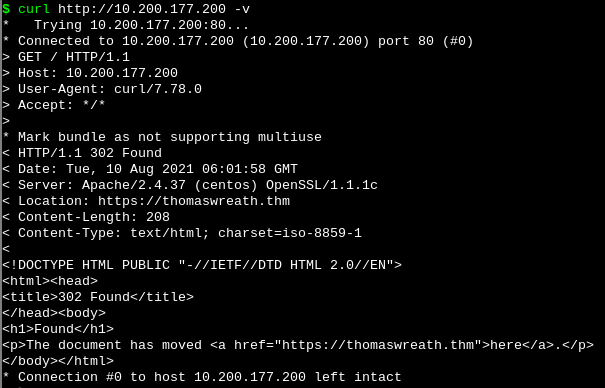
\includegraphics[width=\textwidth]{img/home-redirect.png}

Visiting the page, we only have a static page with nothing exploitable.

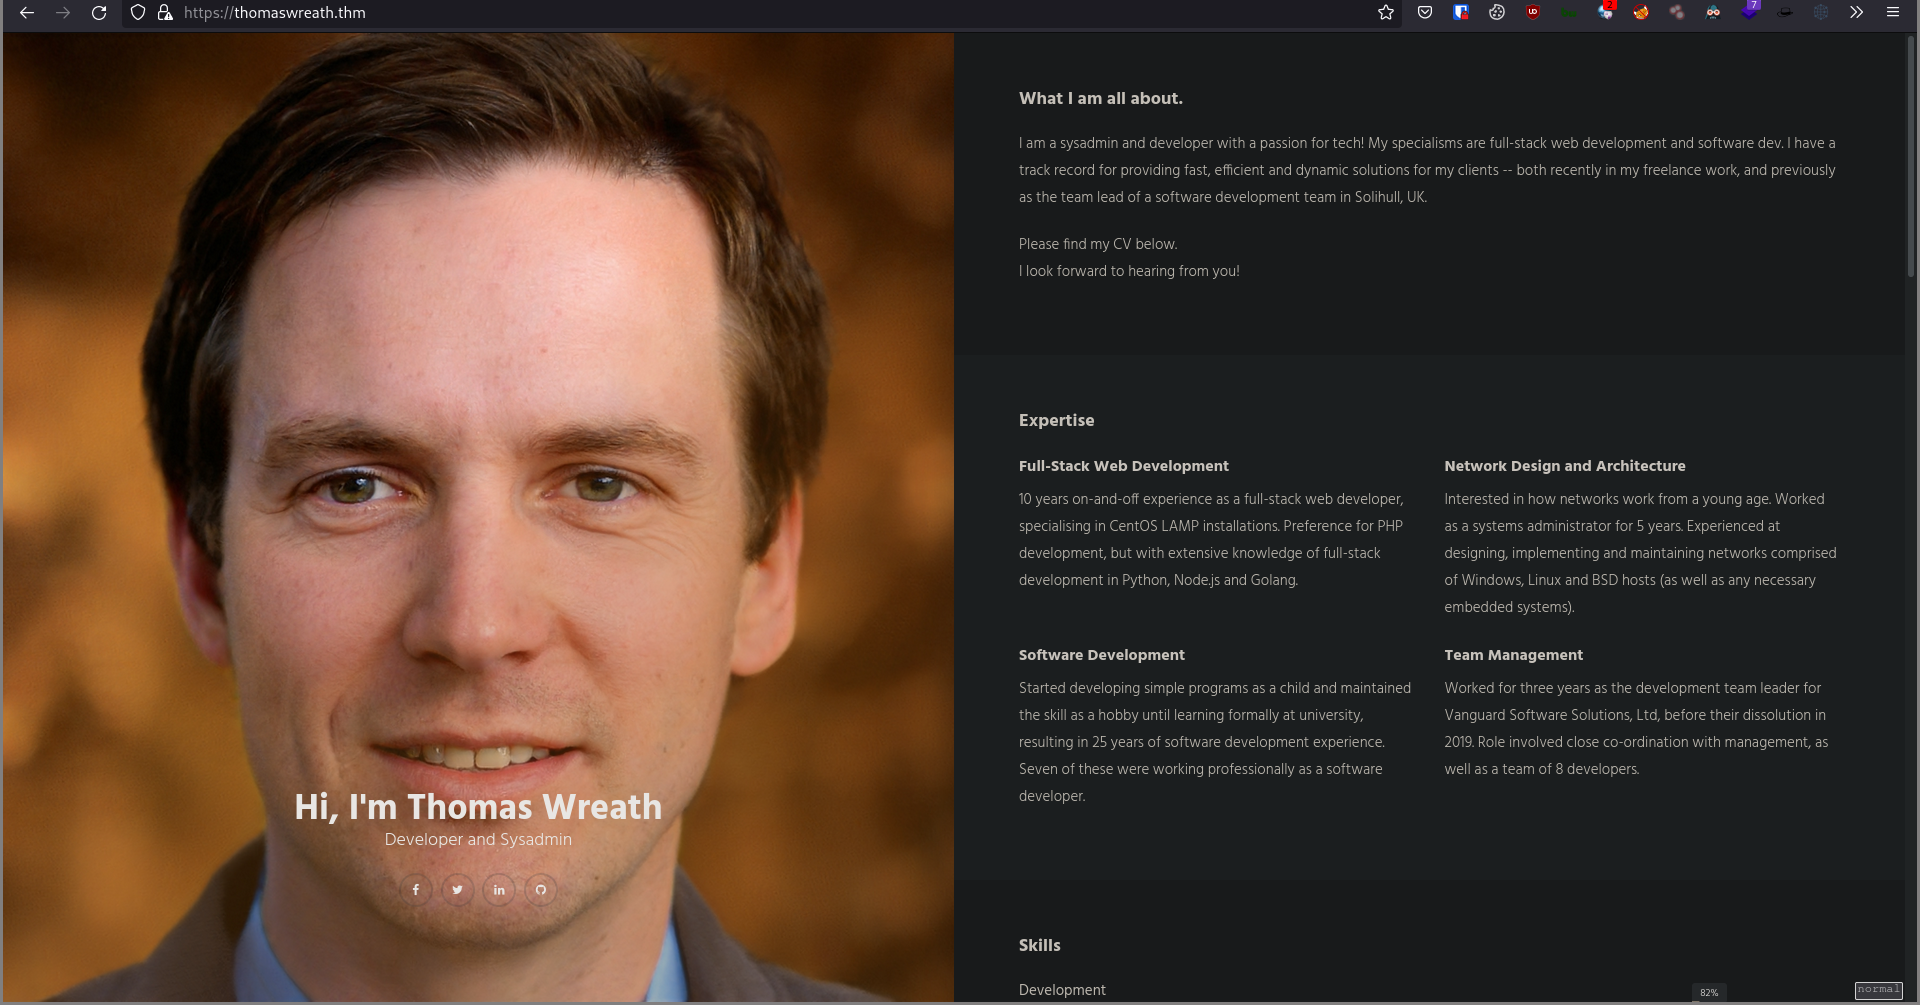
\includegraphics[width=\textwidth]{img/home.png}

The page on port 10000, however, is running an old version of Minserv (1.890) vulnerable to CVE-2019-15107, a Command Injection vulnerability, and has its web server running as root. Therefore, using an pre-made exploit, we can easily gain root access on the server.

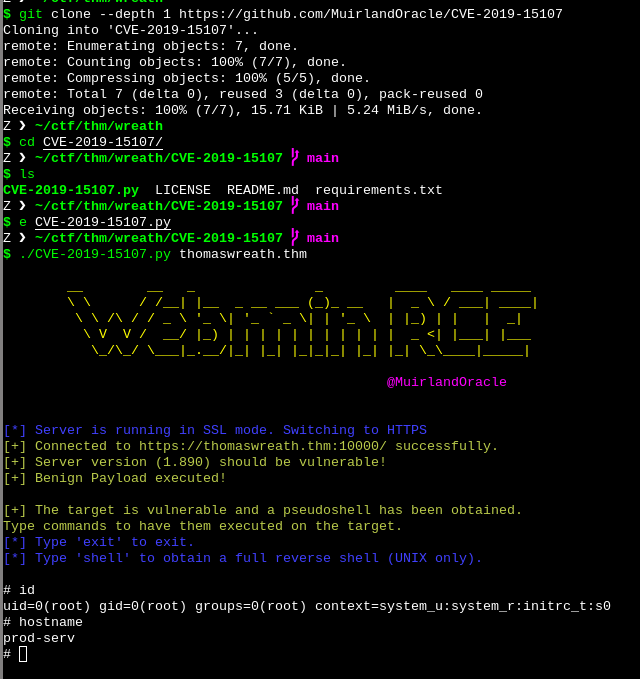
\includegraphics[width=\textwidth]{img/CVE-2019-15107.png}

With root access, I was able to exfiltrate and use root's existing id\_rsa file to impersonate and maintain access as root on prod-serv. After getting a binary of \lstinline{nmap} onto prod-serv, I did an IP scan and found 3 more IP addresses, of which only 10.200.177.100 and 10.200.177.150 are in scope.

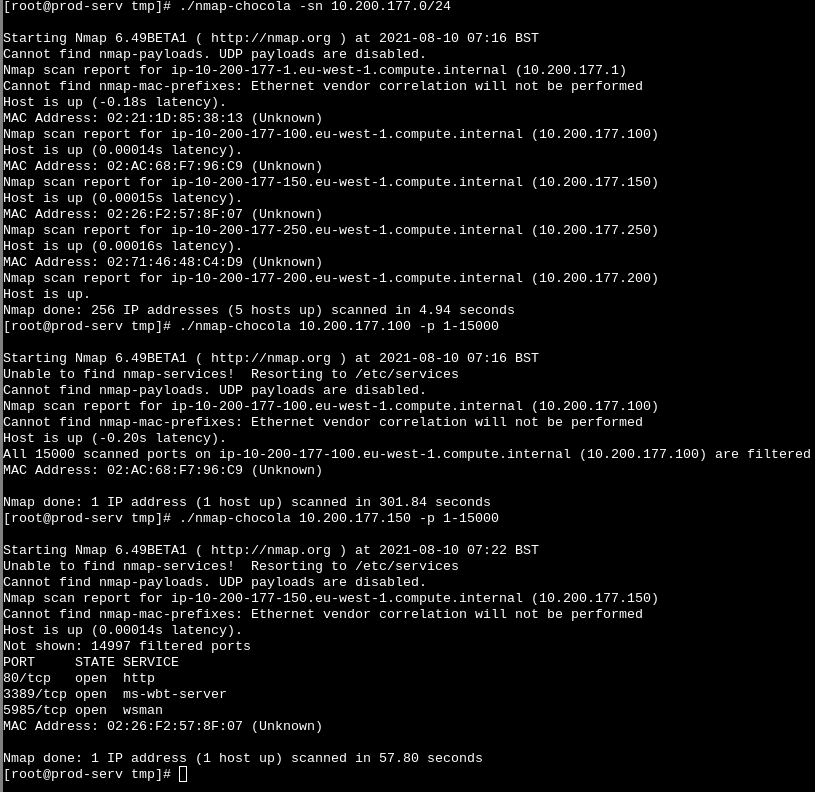
\includegraphics[width=\textwidth]{img/nmap-200.png}

As only 10.200.177.150 has open ports, I went on to enumerate it.

To get access to the internal servers, I ran \lstinline{sshuttle} with the previously found root id\_rsa on prod-serv.

\begin{lstlisting}[basicstyle=\footnotesize]
sshuttle -r root@thomaswreath.thm --ssh-cmd "ssh -i root.prod-serv.ssh" 10.200.177.0/24 -x 10.200.177.200
\end{lstlisting}

With the proxy set up, we're able to go to the web service running on git-serv.

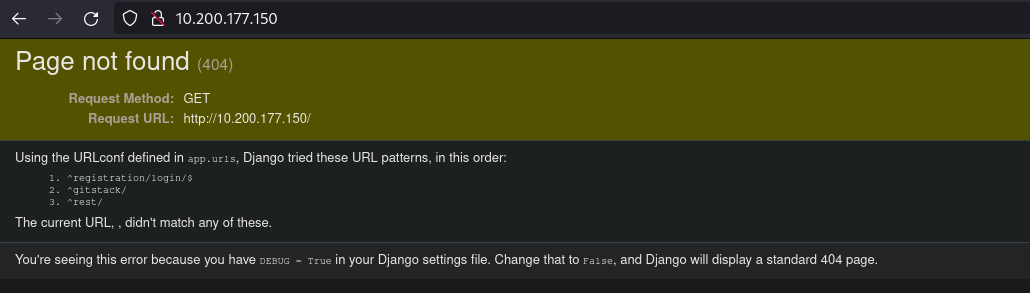
\includegraphics[width=\textwidth]{img/150-home.png}

We can see from the error message that there's a \lstinline{/gitstack} page. Looking for gitstack exploits, we can find exploit \href{https://www.exploit-db.com/exploits/43777}{43777} on Expoit Database. Running this exploit gives us a backdoor, and since the web service is running as "nt authority\textbackslash system", we have access to git-serv as said user.

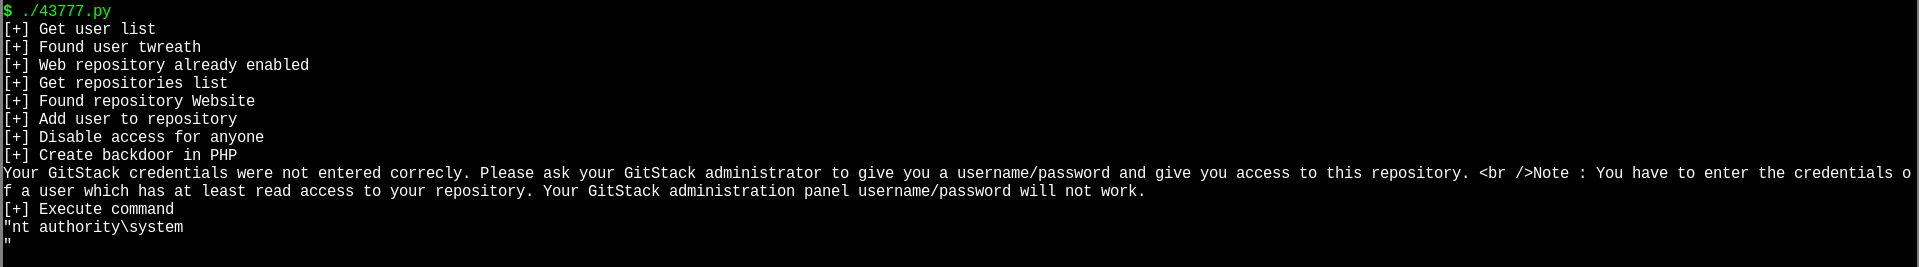
\includegraphics[width=\textwidth]{img/exploit-43777.py.png}

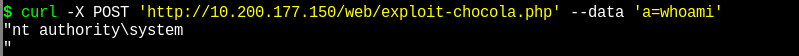
\includegraphics[width=\textwidth]{img/backdoor-43777.py.png}

Because traffic through unused ports are block on prod-serv, I opened port 17171 in the prod-serv's firewall to get a reverse shell on git-serv.

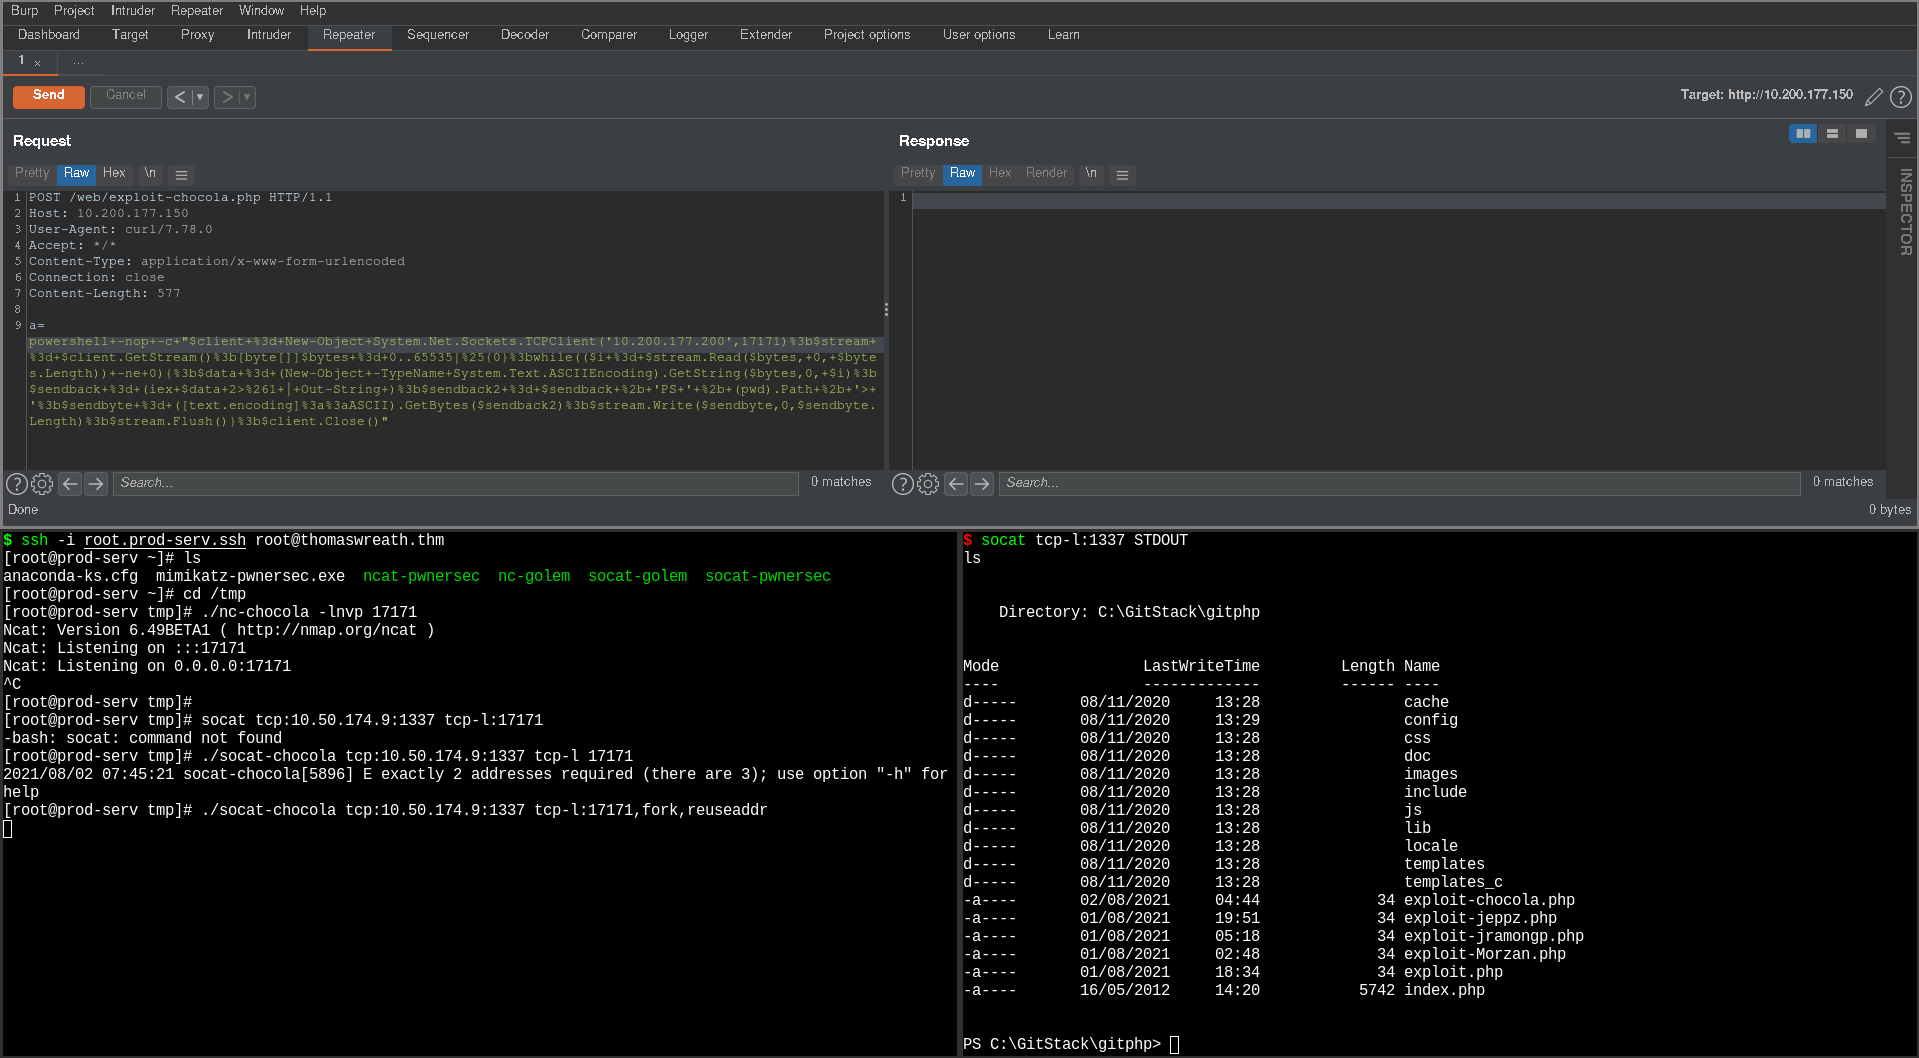
\includegraphics[width=\textwidth]{img/150-revshell.png}

With a shell, I created an Administrative account for persistence, as well as further leverage.

\begin{lstlisting}[basicstyle=\footnotesize]
net user chocola PASSWORD /add
net localgroup Administrators chocola /add
net localgroup "Remote Management Users" chocola /add
\end{lstlisting}

With the backdoor account, I logged in to git-serv through RDP and ran \lstinline{mimikatz} to dump password hashes.

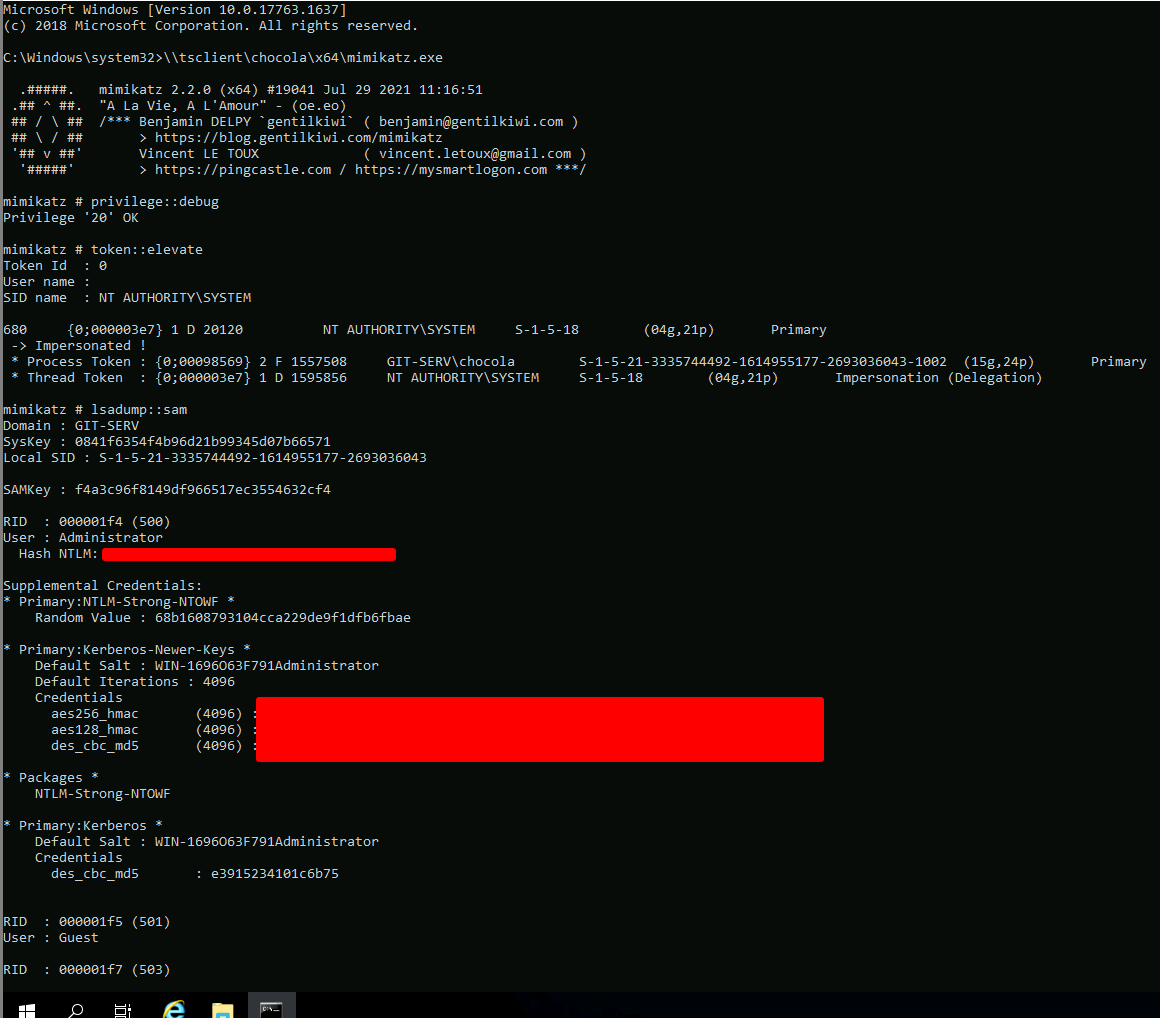
\includegraphics[width=\textwidth]{img/mimikatz.png}

Of the password hashes dumped, only Thomas' password could be cracked. However, I was also able to perform Pass-the-hash with Administrator's hash and get a shell with \lstinline{evil-winrm} as Administrator on git-serv. With this, I found the source code for Mr.Wreath's website on git-serv in \lstinline{C:\textbackslash GitStack\textbackslash repositories\textbackslash website.git}, which we'll come back to later in the report.

Using \href{https://github.com/EmpireProject/Empire/blob/master/data/module_source/situational_awareness/network/Invoke-Portscan.ps1}{Powershell-Empire's Invoke-Portscan} module, I scanned the last remaining machine on 10.200.177.100, and 2 ports were found: 80 and 3389.

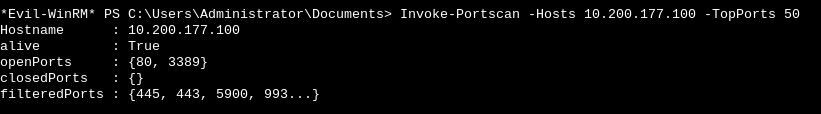
\includegraphics[width=\textwidth]{img/Invoke-Portscan.png}

Looking at the repository found in git-serv, The PHP code in \lstinline{/resources/index.php} is of interest to us.

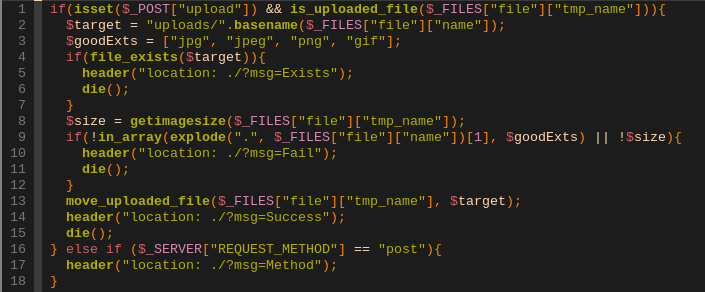
\includegraphics[width=\textwidth]{img/vuln-code.png}

There are 2 filters in place: a file extension whitelist and a image file type check. Regarding the 1st filter, in line 9 of the code above, the file name is split on "." and the 2nd item is checked against  a list of good extensions. This filter can easily be bypassed by having an extra extension in t he file name, for example "file.jpg.php" would pass the filter but still be a PHP file. As for the 2nd filter, it can be passed by uploading a legitimate image file with PHP code somewhere in the file.

To exploit the above vulnerability, a legitimate image file is created that a PHP code execution snippet is inserted as EXIF data, and the malicious image file is then uploaded to the server. This exploit will be used later in the engagement.

In order to reach 10.200.177.100, a hole was opened in git-serv's firewall (port 17171, TCP, inbound) and a binary of chisel was uploaded to git-serv in order to get a proxy. The proxy was acquired as follows:

\begin{lstlisting}
# 10.200.177.150
netsh advfirewall firewall add rule name="chisel-chocola" dir=in action=allow protocol=tcp localport=17171
./chisel-chocola.exe server -p 17171 --socks5

# attacker
chisel client git-serv:17171 9090:socks
\end{lstlisting}

With a proxy, I was able to reach the web server on 10.200.177.100. Going to \lstinline{/resources}, we're met with a Basic auth prompt, for which we can use Thomas' previously cracked credentials. With the previously analyzed file upload vulnerability, I uploaded a malicious image file to the server and got remote code execution.

With the payload on the server, I was able to upload a netcat binary (nc-chocola) to the machine (C:\textbackslash Windows\textbackslash temp\textbackslash nc-chocola.exe) and get a shell as "thomas" on wreath-pc.

With a shell, I then ran \href{https://github.com/carlospolop/PEASS-ng/blob/master/winPEAS/winPEASexe/binaries/Obfuscated\%20Releases/winPEASx64.exe}{winPEAS}. As a result, the service "SystemExplorerHelpService", which was running as Administrator, was found to have an unqoted path.

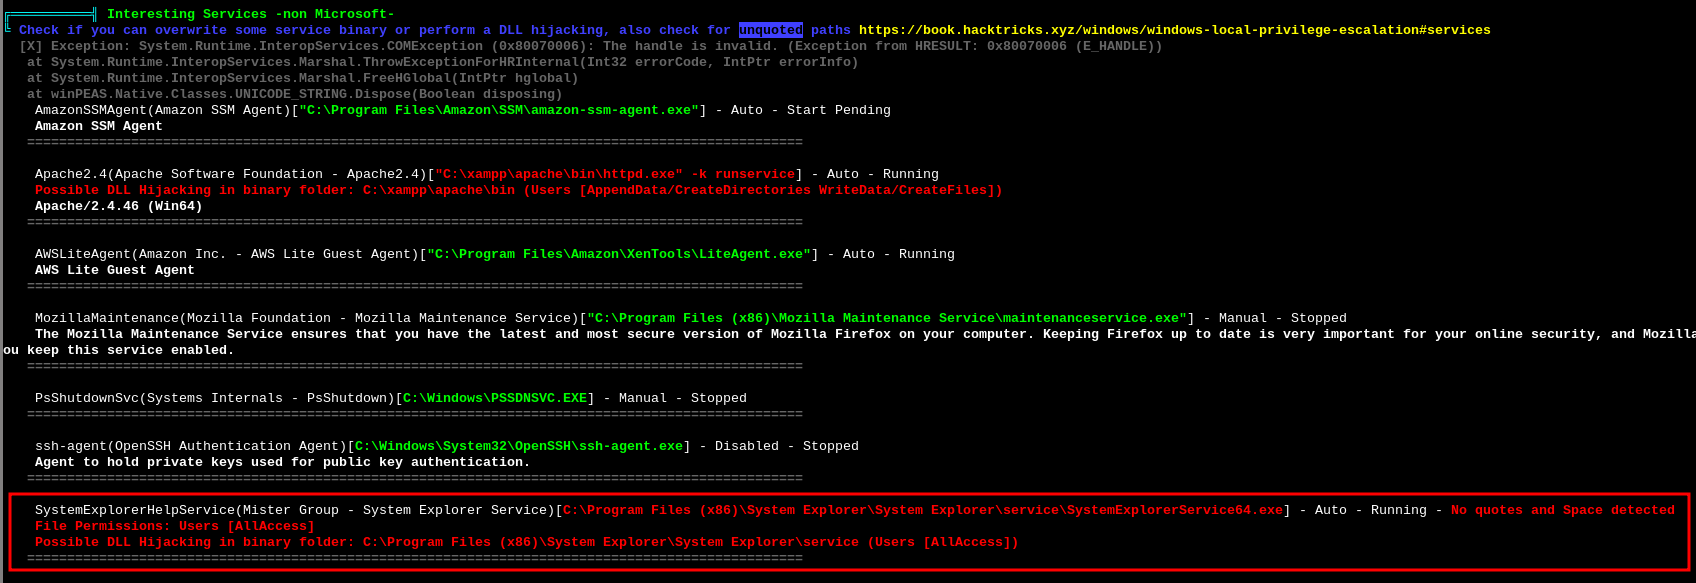
\includegraphics[width=\textwidth]{img/winpeas.png}

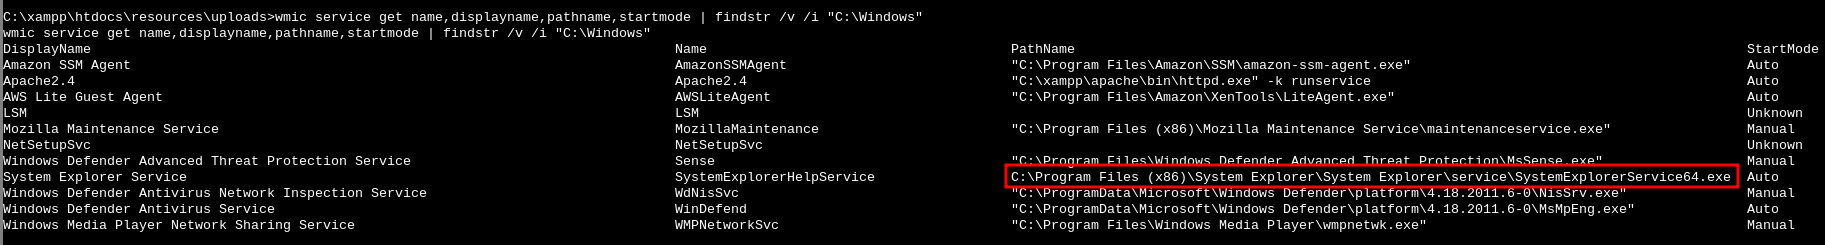
\includegraphics[width=\textwidth]{img/unquoted_service.png}

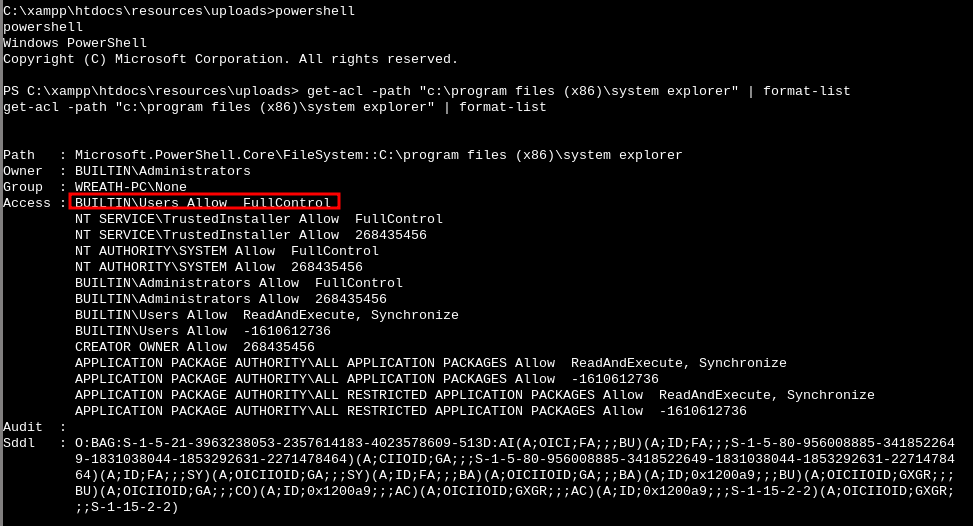
\includegraphics[width=\textwidth]{img/dir_fullcontrol.png}

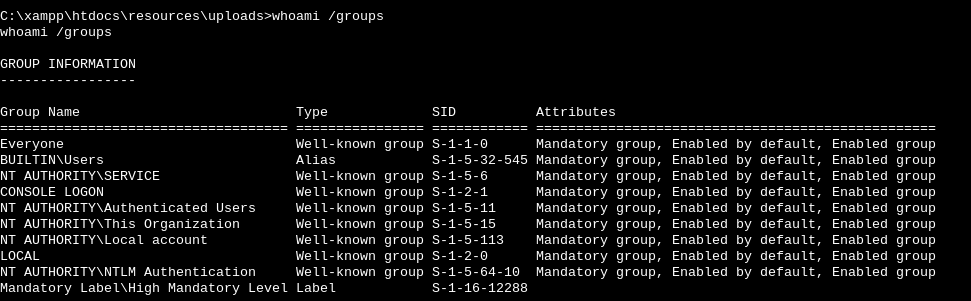
\includegraphics[width=\textwidth]{img/groups.png}

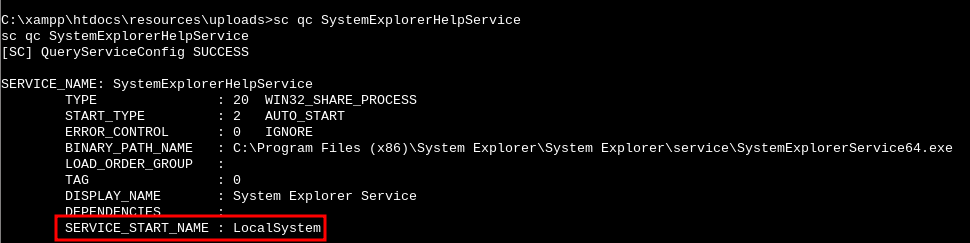
\includegraphics[width=\textwidth]{img/service_as_admin.png}

Additionally, an exploitable path, "C:\textbackslash Program Files (x86)\textbackslash System Explorer\textbackslash System Explorer", was found to have FullControl access by our user, specifically the group "BUILTIN\textbackslash Users". To exploit this, I compiled a wrapper program, whose code is in Appendix 2 (section \ref{appendix-2}, page \pageref{appendix-2}), and placed in on the machine as "C:\textbackslash Program Files (x86)\textbackslash System Explorer\textbackslash System.exe". With this, I was able to exploit the "Unquoted Service Path" vulnerability and get a shell as "nt authority\textbackslash system" on wreath-pc.

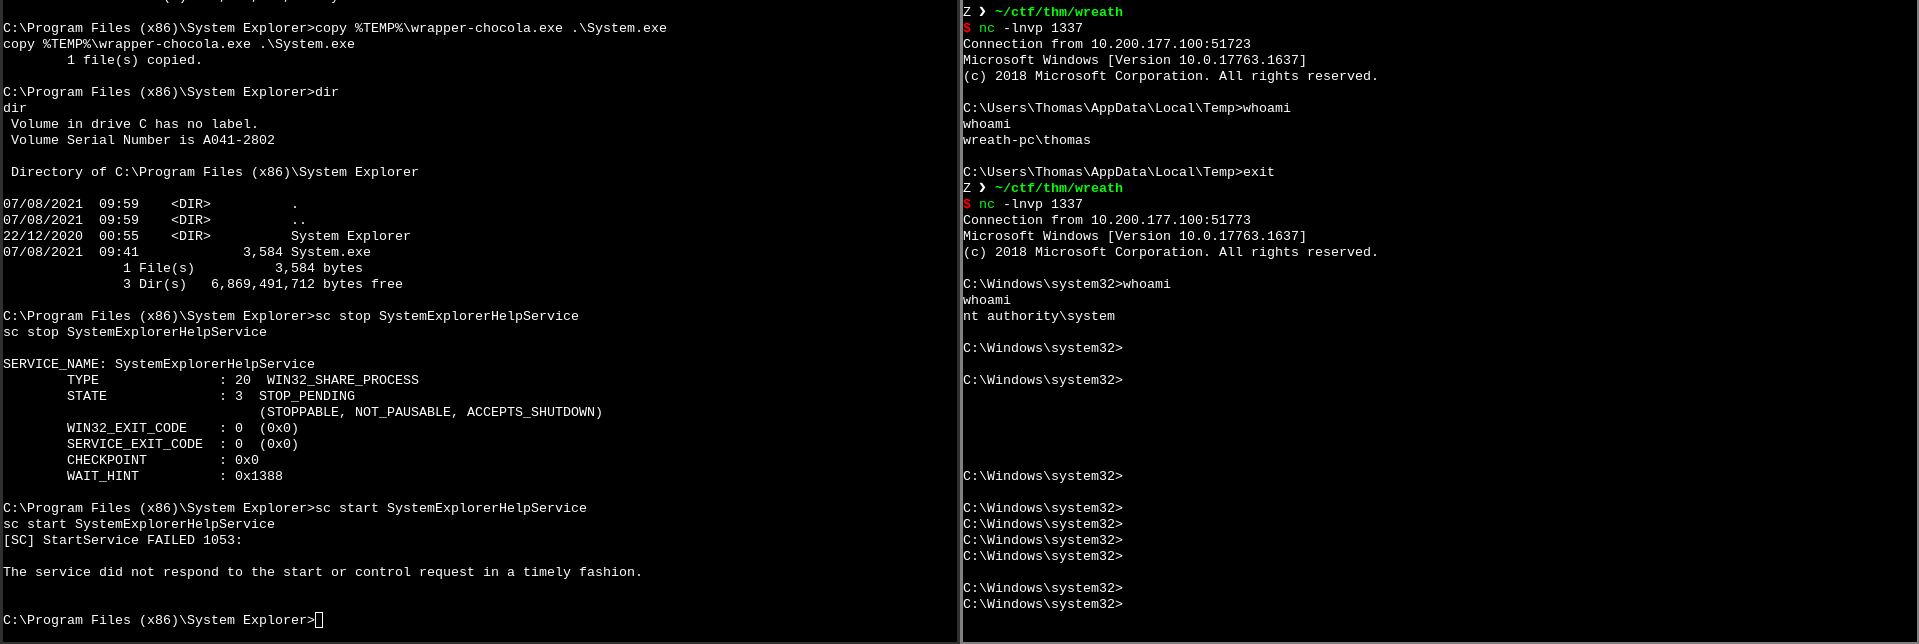
\includegraphics[width=\textwidth]{img/pc-system-shell.png}

With a shell as "nt authority\textbackslash system", I then exfiltrated and dumped password hashes as evidence.

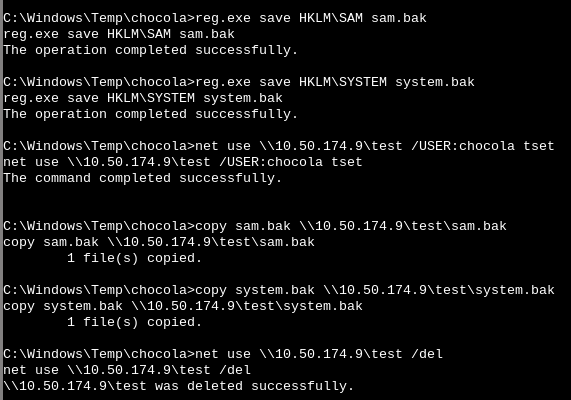
\includegraphics[width=\textwidth]{img/sam_dump.png}

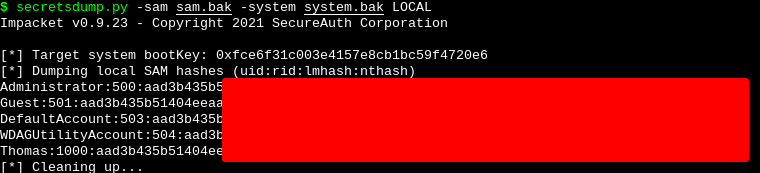
\includegraphics[width=\textwidth]{img/secretsdump.png}
